\section*{Data and Processing}
\addcontentsline{toc}{section}{Data and Processing}

\phantomsection
\subsection*{Data Source and Structure}
\addcontentsline{toc}{subsection}{Data Source and Structure}

    Operated under the oversight of Transport for Ireland (TFI), LUAS real-time tram arrival information is published through an API that sources data from real-time AVLS updates. While this program is accessible via data.gov.ie, historical records are not publicly archived or easily available on request. Directly scraping these logs was not feasible due to the time and computing constraints of this project. Instead, this study makes use of an independently archived dataset compiled by Dublin-based developer Eoin O’Brien, who has collected continuous forecast logs from the API referenced above, spanning January 2020 to October 2022 \parencite{obrien2022historical}. When contacted, and on his website, O’Brien mentioned no restrictions on academic use and expressed support for its inclusion in this study. Furthermore, as only publicly available, non-identifiable AVLS data is used, no personal or private information was accessed, meeting ethical requirements.

    This dataset contains timestamped forecast records of all upcoming tram arrivals, logged approximately every two minutes, across all LUAS stations and lines. In total, it comprises over 160 million rows, providing a comprehensive view of the system’s behaviour over time. Given the size and regularity of logging, records were processed into time-based \texttt{ServiceDay} groupings to enable scalable batch processing, more efficient validation, and robust temporal analysis. This field also ensured complete journeys, as the operational schedule runs from around 5:30 am to 12:30 am, ensuring the inclusion of trams running past midnight, into the following calendar day \parencite{tfi_luas}. Additional processing was performed to extract time-of-day categories: morning, midday, evening, and night.

    The key columns extracted and used for reconstruction and analysis were:

\begin{itemize}
  \item \texttt{DateTime}: the timestamp of the forecast; standardised via \texttt{timedelta}
  \item \texttt{Origin}: the station at which the forecast was recorded; renamed \texttt{Stop} for clarity
  \item \texttt{Line}: the major route of the station; \texttt{Red} or \texttt{Green}
  \item \texttt{Direction}: the tram trajectory; \texttt{Inbound} (North/East) or \texttt{Outbound} (South/West)
  \item \texttt{Minutes}: the number of minutes forecasted until arrival at the stop
  \item \texttt{Destination}: the scheduled end terminus of the tram
  \item \texttt{ServiceDay}: the operational date of the service taken from \texttt{DateTime}
  \item \texttt{Period}: the time of day the forecast occurs, calculated from \texttt{DateTime}
\end{itemize}

\phantomsection
\subsection*{Pandemic Phase Segmentation}
\addcontentsline{toc}{subsection}{Pandemic Phase Segmentation}

    A major factor in processing was the need to account for the impact of the COVID-19 pandemic; to reflect how this evolving public health emergency affected operations, the data was segmented into distinct phases based on major policy milestones. Although the Irish Government officially implemented national restrictions on March 27, 2020, under the Health Act 2020, the pre-COVID phase ends slightly ahead of the official lockdown date to account for anticipatory behavioural shifts and early institutional responses \parencites{govireland2020a}{govireland2020b}. Gradual reopening at the end of May 2021 introduced what was widely referred to as the "new normal,” though this phase still involved capacity limits, vaccination certification, and intermittent restrictions \parencite{govireland2021}. The final removal of public health restrictions in January 2022 marked the beginning of a post-pandemic phase of near-normalised operations \parencites{govireland2022}{depthealth2022}.

    Accordingly, the dataset is divided into four phases for comparative analysis:

\begin{itemize}
  \item \textbf{Pre-COVID}: 20 January 2020 to 20 March 2020
  \item \textbf{Lockdown}: 21 March 2020 to 31 May 2021
  \item \textbf{Recovery}: 1 June 2021 to 21 January 2022
  \item \textbf{Post-COVID}: 22 January 2022 to 22 October 2022
\end{itemize}

\phantomsection
\subsection*{Stop Templates}
\addcontentsline{toc}{subsection}{Stop Templates}

\begin{figure}[H]
  \centering
  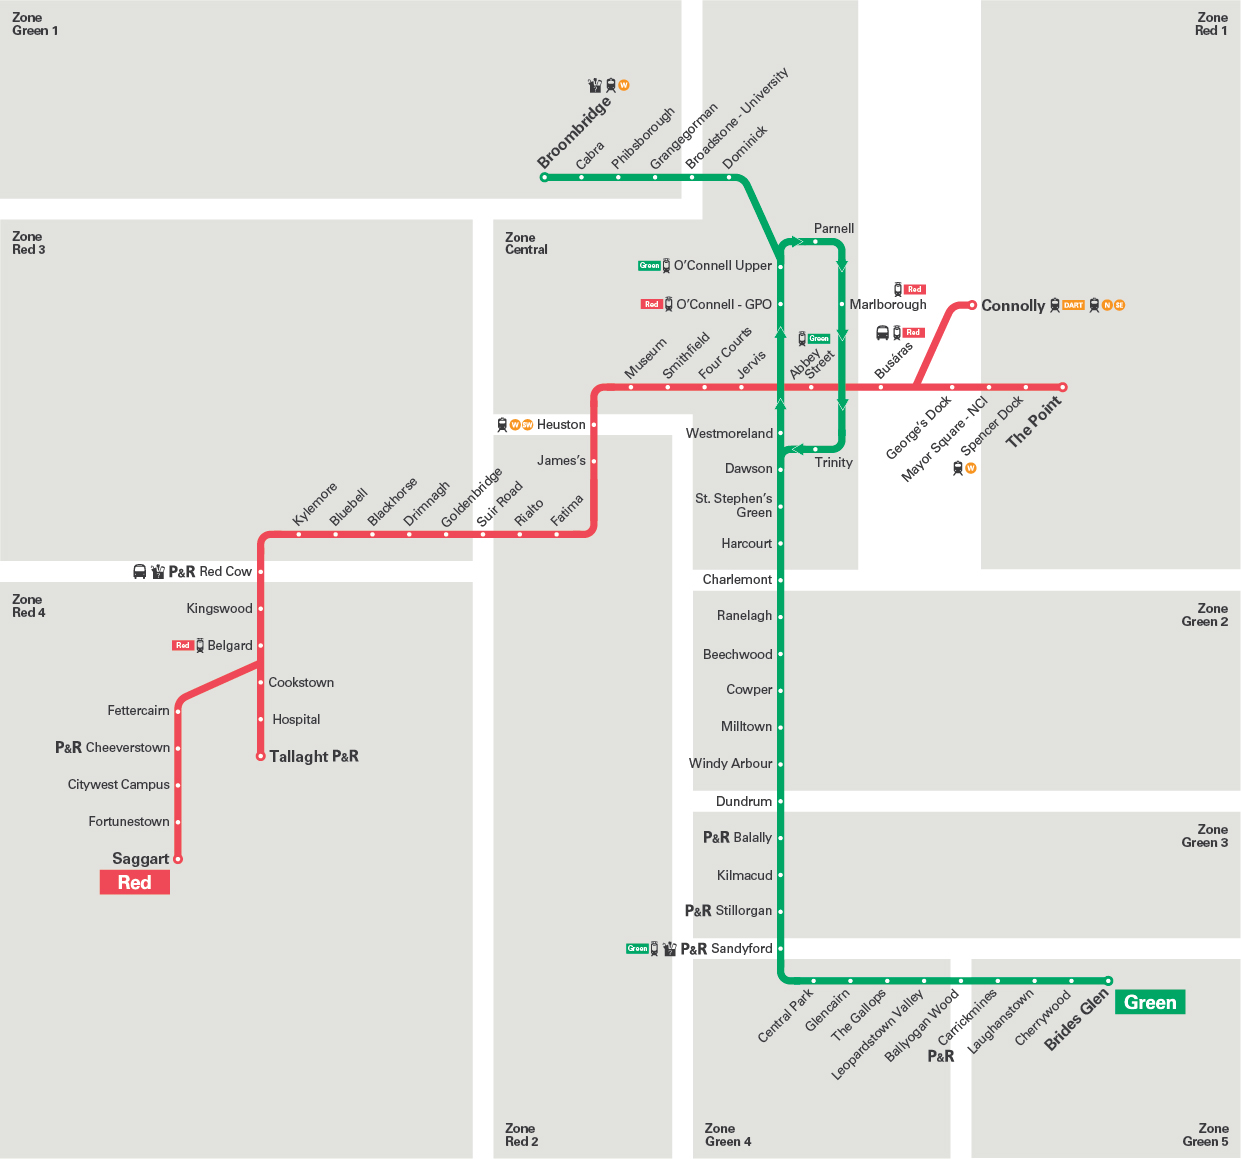
\includegraphics[width=0.6\textwidth]{figures/paper_figures/station_map.jpg}
  \caption{LUAS Station Routes. Source: Transport for Ireland}
  \label{fig:luas_routes}
\end{figure}

    To facilitate the stitching of full tram journeys, a dictionary of stop templates was created to reflect the sequential order of LUAS stops along each route. These initially mirrored standard full-service patterns for both lines, seen in Figure~\ref{fig:luas_routes}, and served as a reference for identifying valid progressions within the forecast snapshot data. This approach ensured that only plausible directional sequences were linked, helping to reduce errors from route anomalies or forecast noise.

    However, during early exploration, it became clear that some snapshots terminated unexpectedly at intermediate stops, typically Dominick or Connolly; these truncated journeys were not necessarily indicative of data error but reflected real-world operational constraints like city centre disruptions, partial routings, or planned diversions. Rather than discard these cases, the stop templates were expanded to include any recurring endpoints that appeared with sufficient frequency. This adaptive strategy allowed for a more accurate reconstruction of service behaviour by acknowledging that not all trams span the entire route.  Using this approach, over 375,000 valid tram journeys were reconstructed across both lines and directions from January 2020 to October 2022, capturing not just full-route trips but also consistent partial services. The result was a consistent and flexible matching process that captured the actual behaviour of LUAS vehicles, avoiding assumptions about completion while maintaining logical structure.
    
    This study intentionally grounded stop templates solely on destination-based endpoints, rather than attempting to infer full start-to-end routes from partial data. By focusing only on observable destinations, defined by significant stations seen in end destination counts, speculative reconstruction of full routes and potential data overfitting was avoided. The handling of non-traditional terminus journeys was important in capturing irregular or truncated services caused by disruption, without introducing errors from falsely completed journeys. Using destination frequency as a filtering mechanism ensured that the templates remained representative of real operational patterns, further ensuring the building process was tractable and replicable. However, as the approach relies on periodic forecasts rather than continuous tracking, some journeys may be over- or under-segmented, particularly during peak congestion or when data gaps occur between snapshots. Given the nature of forecast data, exact route replication was never expected; instead, the reconstruction prioritised internal consistency and behavioural plausibility over fine-grained precision.



    \phantomsection
\subsection*{Analytical Limitations and Design Decisions}
\addcontentsline{toc}{subsection}{Analytical Limitations and Design Decisions}

    A significant limitation of this study was the absence of unique tram vehicle identifiers in the forecast dataset. Without access to vehicle IDs, it was not possible to definitively track individual trams as they moved through the network; this became particularly challenging in high-frequency segments, where multiple trams might serve the same direction within a short time frame. To address this, trams were reconstructed using sequential station-based inference, guided by forecasted arrival timestamps and directional stop templates, allowing for the approximation of tram movement across the network without overcomplicating the stitching process. Temporal filters helped prevent implausible overlaps, particularly during peak periods, further maintaining the integrity of the inferred journeys even in the absence of direct vehicle tracking. Due to these constraints, the focus of the analysis shifted toward broader route-level dependability rather than specific operations. While this approach restricts the ability to evaluate factors such as inter-trip recovery or tram-specific consistency, it remains aligned with the passenger perspective of reliability, which is primarily shaped by observed spacing, journey duration, and scheduling at the station level.

    A further methodological decision was the exclusion of the Status Message field provided in API logs. Although these messages occasionally offered useful context on disruptions, their lack of standardisation, inconsistent phrasing, and absence of structured metadata limited their analytical value. Incorporating them would have required subjective interpretation or manual parsing, creating potential risks of introducing noise or misclassification. As a result, stops were assumed to be active unless indicated otherwise in the log structure, acknowledging that some inferred journeys may include segments that were operationally bypassed but still could have been logged by the AVLS system. In cases where sequences terminated early or deviated from full-route templates, the data was not treated as erroneous; instead, recurring truncated journeys were accepted as legitimate service patterns, with acknowledgement of partial operations due to diversions, disruptions, or modified timetables. This decision was consistent with the study’s overarching principle of prioritising observed system behaviour over assumed norms. While this may occasionally include non-revenue or non-passenger movements, it ensures that the analysis captures the full scope of operational irregularities rather than smoothing through strict filtering.

    Finally, the high temporal resolution, with forecasts recorded every two minutes, and sheer scale of over 160 million rows introduced inherent limitations for capturing stop-level events with exact precision. Some arrivals or departures may have occurred between snapshot intervals, potentially leading to under- or over-representation of certain events. However, given the volume and consistency of the logs, averaged over varying periods and phases, this granularity was deemed sufficient for identifying broader service patterns and supporting the computation of regularity across the network.